\documentclass[aspectratio=169,11pt,hyperref={bookmarks=false}]{beamer}

\usetheme{Madrid}
\usecolortheme{default}

\definecolor{MarketBlue}{RGB}{28,73,128}
\definecolor{MarketGreen}{RGB}{20,120,90}
\definecolor{MarketRed}{RGB}{170,55,55}
\definecolor{MarketAmber}{RGB}{180,115,20}

\setbeamercolor{structure}{fg=MarketBlue}
\setbeamercolor{title}{fg=white,bg=MarketBlue}
\setbeamercolor{frametitle}{fg=white,bg=MarketBlue}
\setbeamercolor{block title}{fg=white,bg=MarketBlue}
\setbeamercolor{block body}{bg=blue!4}
\setbeamertemplate{navigation symbols}{}
\setbeamertemplate{footline}{}

\usepackage{booktabs}
\usepackage{tabularx}
\usepackage{array}
\usepackage{tikz}
\usetikzlibrary{arrows.meta,positioning,shapes.geometric}

\newcommand{\smallsep}{\vspace{0.35em}}
\newcommand{\good}[1]{\textcolor{MarketGreen}{#1}}
\newcommand{\warn}[1]{\textcolor{MarketAmber}{#1}}
\newcommand{\risk}[1]{\textcolor{MarketRed}{#1}}

\title[MarketGyan]{MarketGyan: NEPSE-Impact Dataset, Model Results, and RAG Demo Progress}
\author{Bikash Kumar Sah}
\institute{Project Supervisor Discussion}
\date{June 21, 2026}

\begin{document}

\begin{frame}
  \titlepage
\end{frame}

\begin{frame}{Project Goal}
  \begin{block}{Research contribution}
    MarketGyan builds a Nepal-specific benchmark and modeling workflow for deciding whether news is relevant to NEPSE, mapping it to sectors and listed symbols, and producing evidence-grounded market-impact labels.
  \end{block}
  \smallsep
  \begin{itemize}
    \item Core dataset: human-adjudicated bilingual \textbf{NEPSE-Impact-500}.
    \item Modeling: XLM-R baseline, FinBERT English subset baseline, and Qwen3-8B QLoRA experiment.
    \item Runtime principle: current market facts come from deterministic data and RAG, not from model memory.
    \item Output boundary: informational analysis only, never investment advice or trading signals.
  \end{itemize}
\end{frame}

\begin{frame}{Why the Problem Was Reframed}
  \begin{columns}[T]
    \begin{column}{0.49\textwidth}
      \begin{block}{What failed in the first idea}
        General business news looked financial but often had no defensible NEPSE impact mechanism.
      \end{block}
      \begin{itemize}
        \item Non-listed company announcements
        \item Product promotions and workshops
        \item Foreign business or technology news
        \item Broad economy stories without market linkage
      \end{itemize}
    \end{column}
    \begin{column}{0.49\textwidth}
      \begin{block}{Revised task}
        Teach the model Nepal-market relevance, event taxonomy, entity mapping, and evidence selection.
      \end{block}
      \begin{itemize}
        \item Direct listed-company or market impact
        \item Indirect sector or macro mechanism
        \item Hard-negative general business examples
      \end{itemize}
    \end{column}
  \end{columns}
\end{frame}

\begin{frame}{Novelty Position}
  \small
  \begin{tabularx}{\textwidth}{@{}p{0.23\textwidth}X@{}}
    \toprule
    Reference idea & MarketGyan contribution \\
    \midrule
    FinBERT & Domain adaptation, but focused on Nepal market relevance instead of generic English finance sentiment. \\
    FinGPT & Data-centric lightweight tuning using a local, auditable, human-reviewed finance corpus. \\
    FinLLM survey & Benchmark design with hallucination, validity, grounding, language, and event-category metrics. \\
    FinTral & Multi-task financial instruction tuning with structured labels, sectors, symbols, and evidence. \\
    \bottomrule
  \end{tabularx}
  \smallsep
  \begin{block}{Supervisor-facing claim}
    LoRA is not the novelty. The novelty is the NEPSE-specific ontology, bilingual benchmark, adjudication workflow, and evidence-grounded evaluation.
  \end{block}
\end{frame}

\begin{frame}{End-to-End Data Pipeline}
  \centering
  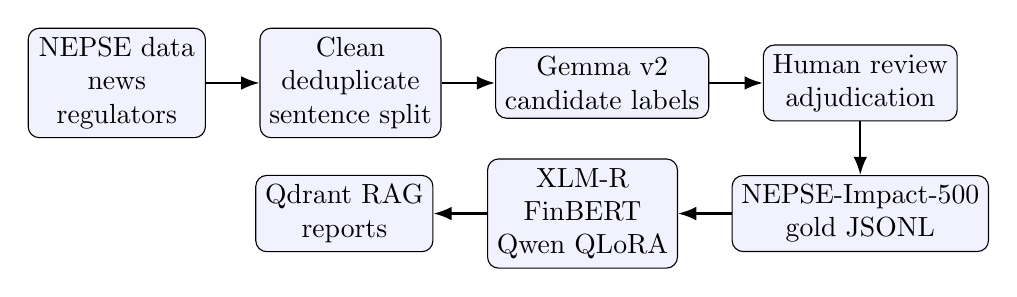
\begin{tikzpicture}[
    node distance=0.68cm,
    box/.style={draw, rounded corners, align=center, minimum width=2.25cm, minimum height=0.74cm, fill=blue!5},
    arrow/.style={-Latex, thick}
  ]
    \node[box] (sources) {NEPSE data\\news\\regulators};
    \node[box, right=of sources] (clean) {Clean\\deduplicate\\sentence split};
    \node[box, right=of clean] (gemma) {Gemma v2\\candidate labels};
    \node[box, right=of gemma] (review) {Human review\\adjudication};
    \node[box, below=of review] (gold) {NEPSE-Impact-500\\gold JSONL};
    \node[box, left=of gold] (models) {XLM-R\\FinBERT\\Qwen QLoRA};
    \node[box, left=of models] (rag) {Qdrant RAG\\reports};
    \draw[arrow] (sources.east) -- (clean.west);
    \draw[arrow] (clean.east) -- (gemma.west);
    \draw[arrow] (gemma.east) -- (review.west);
    \draw[arrow] (review.south) -- (gold.north);
    \draw[arrow] (gold.west) -- (models.east);
    \draw[arrow] (models.west) -- (rag.east);
  \end{tikzpicture}
  \smallsep
  \begin{itemize}
    \item Numeric market snapshots are deterministic and stored with provenance.
    \item Gemma is only a teacher candidate generator; human adjudication creates gold labels.
  \end{itemize}
\end{frame}

\begin{frame}{Corpus Status: NEPSE-Impact-500}
  \small
  \begin{tabularx}{\textwidth}{@{}lrrX@{}}
    \toprule
    Component & Count & Status & Purpose \\
    \midrule
    Gold records & 500 & \good{Ready} & Training and evaluation dataset. \\
    Direct records & 300 & \good{Target met} & Listed company or market impact. \\
    Indirect records & 100 & \good{Target met} & Sector or macro mechanism. \\
    Hard negatives & 100 & \good{Target met} & Business news without NEPSE mechanism. \\
    English records & 299 & \good{Target met} & English benchmark coverage. \\
    Nepali records & 200 & \good{Target met} & Nepali benchmark coverage. \\
    Symbol-level records & 273 & \good{Target met} & Listed-company mapping task. \\
    \bottomrule
  \end{tabularx}
  \smallsep
  \begin{block}{Quality control}
    Duplicate groups are isolated in splits; records retain source URL, date, candidate label, human label, and evidence sentence IDs.
  \end{block}
\end{frame}

\begin{frame}{Ontology and Gold Label}
  \begin{columns}[T]
    \begin{column}{0.50\textwidth}
      \begin{block}{Classification fields}
        \begin{itemize}
          \item Relevance: direct, indirect, not relevant
          \item Event type
          \item Impact scope
          \item Impact direction
          \item Impact horizon
          \item Impact mechanism
        \end{itemize}
      \end{block}
    \end{column}
    \begin{column}{0.47\textwidth}
      \begin{block}{Grounding fields}
        \begin{itemize}
          \item NEPSE sector names
          \item Listed symbols
          \item Confidence band
          \item Evidence sentence IDs
          \item Source metadata and URL
        \end{itemize}
      \end{block}
    \end{column}
  \end{columns}
  \smallsep
  \begin{block}{Annotation rule}
    A positive label requires a concrete NEPSE company, sector, market, regulatory, liquidity, or macroeconomic mechanism.
  \end{block}
\end{frame}

\begin{frame}{Current Baseline Results}
  \small
  \begin{tabularx}{\textwidth}{@{}lccX@{}}
    \toprule
    Model/task & Accuracy & Macro-F1 & Interpretation \\
    \midrule
    XLM-R relevance & 0.787 & 0.723 & Current dependable relevance baseline. \\
    XLM-R direction & 0.683 & 0.549 & Usable, but direction classes still need more data. \\
    FinBERT English direction & 0.889 & 0.616 & Strong on small English relevant subset; not bilingual. \\
    Qwen3 QLoRA v3 strict & 0.333 & 0.384 & Failed official strict-output gate. \\
    \bottomrule
  \end{tabularx}
  \smallsep
  \begin{block}{Current conclusion}
    XLM-R is the strongest reliable classifier. Qwen is still a research experiment until strict JSON validity and evidence grounding improve.
  \end{block}
\end{frame}

\begin{frame}{Qwen3-8B QLoRA: What We Learned}
  \small
  \begin{tabularx}{\textwidth}{@{}lccX@{}}
    \toprule
    Metric & Strict v3 & Tolerant diagnostic & Meaning \\
    \midrule
    JSON validity & 36.0\% & 68.0\% & Many outputs are near-valid, not production-valid. \\
    Evidence grounding & 36.0\% & 68.0\% & Sentence IDs improve only after repair. \\
    Relevance macro-F1 & 0.384 & 0.555 & The adapter learned some relevance signal. \\
    Direction macro-F1 & 0.413 & 0.629 & Direction extraction is promising but not deployable. \\
    Symbol F1 & -- & 0.790 & Entity extraction is the strongest Qwen signal. \\
    Evidence F1 & -- & 0.633 & Evidence selection still needs control. \\
    \bottomrule
  \end{tabularx}
  \smallsep
  \begin{block}{Important boundary}
    Tolerant repair is failure analysis only. It does not count as official validity or deployment readiness.
  \end{block}
\end{frame}

\begin{frame}{Why Qwen Is Not Ready Yet}
  \begin{itemize}
    \item Fine-tuning raises the probability of schema-like text but cannot guarantee JSON.
    \item The model often emits unquoted keys, Markdown/prose, repeated IDs, or non-canonical enums.
    \item Nepali and hard-negative examples remain more difficult than direct English finance news.
    \item Runtime use needs schema-constrained decoding through vLLM or an OpenAI-compatible JSON Schema path.
  \end{itemize}
  \smallsep
  \begin{block}{Decision}
    Keep Qwen as a compact classifier/extractor. Do not use it as a free-form post-market report writer.
  \end{block}
\end{frame}

\begin{frame}{RAG and Report Generation Design}
  \centering
  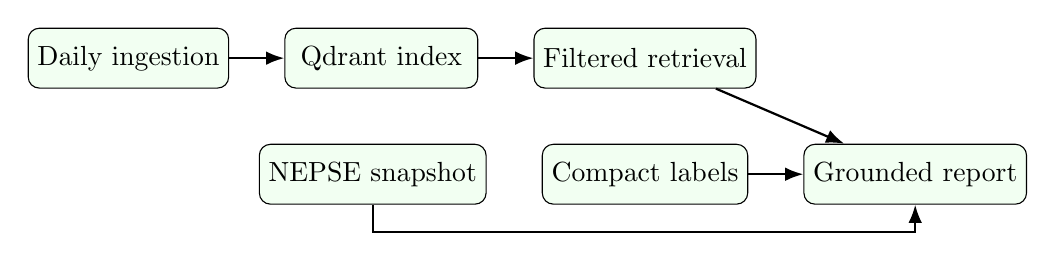
\begin{tikzpicture}[
    node distance=0.7cm,
    box/.style={draw, rounded corners, align=center, minimum width=2.45cm, minimum height=0.76cm, fill=green!5},
    arrow/.style={-Latex, thick}
  ]
    \node[box] (ingest) {Daily ingestion};
    \node[box, right=of ingest] (index) {Qdrant index};
    \node[box, right=of index] (retrieve) {Filtered retrieval};
    \node[box, below=of retrieve] (label) {Compact labels};
    \node[box, left=of label] (snapshot) {NEPSE snapshot};
    \node[box, right=of label] (report) {Grounded report};
    \draw[arrow] (ingest) -- (index);
    \draw[arrow] (index) -- (retrieve);
    \draw[arrow] (retrieve) -- (report);
    \draw[arrow] (label) -- (report);
    \draw[arrow] (snapshot.south) -- ++(0,-0.35) -| (report.south);
  \end{tikzpicture}
  \smallsep
  \begin{block}{Citation rule}
    Sentence IDs are internal anchors only. User-facing reports must show source title, URL, date, chunk ID, content hash, and exact evidence text.
  \end{block}
  \begin{block}{Demo-safe mode}
    A deterministic FastAPI mock agent can build answers and reports from retrieved Qdrant citations while Qwen remains disabled for runtime claims.
  \end{block}
\end{frame}

\begin{frame}{Implemented Demo Workspace}
  \small
  \begin{tabularx}{\textwidth}{@{}p{0.27\textwidth}X@{}}
    \toprule
    UI area & Current behavior \\
    \midrule
    Overview & Snapshot mini-cards, sector/story placeholders, latest report summary, disclaimer. \\
    Ask MarketGyan & Grounded Q\&A with filters, citations, disclaimer, and fail-closed errors. \\
    Evidence Search & Qdrant search with source URLs, scores, sectors, symbols, and sentence anchors. \\
    Reports & Latest published report, citation cards, and local-only generation control. \\
    System & Runtime readiness checklist with safe booleans only; no secrets exposed. \\
    Validate data & Local-review tab remains available only when review API is enabled. \\
    \bottomrule
  \end{tabularx}
  \smallsep
  \begin{block}{Recent UI hardening}
    Forms are disabled when runtime status is unavailable, report generation blocks future dates, and snapshot metrics no longer collide visually.
  \end{block}
\end{frame}

\begin{frame}{Current Demonstration Path}
  \begin{enumerate}
    \item Show NEPSE-Impact-500 and the schema-v2 ontology.
    \item Show XLM-R, FinBERT, and Qwen v3 results with the strict-output limitation.
    \item Start Qdrant and index MarketGyan evidence.
    \item Start Node backend with query and review flags enabled.
    \item Start FastAPI agent in deterministic mock mode.
    \item Use the dashboard: Evidence Search, Ask MarketGyan, Reports, and System.
    \item Verify every answer/report includes citations and the disclaimer.
  \end{enumerate}
\end{frame}

\begin{frame}{Remaining Work}
  \begin{enumerate}
    \item Complete second-review agreement on 110 stratified records.
    \item Evaluate at least 30 retrieval queries and 20 report/query scenarios.
    \item Add schema-constrained Qwen decoding for runtime-style evaluation.
    \item Decide whether Qwen is a positive result or negative experiment.
    \item Improve direction-class coverage if final model metrics are weak.
    \item Run the final supervisor demo with Qdrant, Node, FastAPI, and React.
  \end{enumerate}
  \smallsep
  \begin{block}{Deployment gate}
    Runtime Qwen use remains disabled unless strict JSON validity and evidence grounding reach at least 95\%.
  \end{block}
\end{frame}

\begin{frame}{Supervisor Discussion Points}
  \begin{block}{What is complete}
    Data pipeline, ontology, 500 adjudicated records, baseline experiments, Qwen v3 failure analysis, RAG citation design, FastAPI mock agent, and full dashboard demo workspace.
  \end{block}
  \begin{block}{What needs feedback}
    Whether to present Qwen as a negative experiment unless constrained decoding passes, and how much second-review agreement is required before final submission.
  \end{block}
  \begin{block}{Core message}
    MarketGyan is an evidence-grounded Nepal market-impact benchmark and demo system, not a prediction engine or investment-advice tool.
  \end{block}
\end{frame}

\end{document}
